% Afficher des recommendations concernant la syntaxe.
\RequirePackage[orthodox,l2tabu]{nag}
\RequirePackage{luatex85}
% Paramètres du document.
\documentclass[%
a4paper%                       Taille de page.
,fontsize=17pt%                Taille de police.
,DIV=17%                       Plus grand => des marges plus petites.
,titlepage=off%                Faut-il une page de titre ?
,headings=optiontoheadandtoc%  Effet des paramètres optionnels de section.
,headings=small%
,parskip=false%
,openany%
]{scrbook}
\renewcommand*\partheademptypage{\thispagestyle{empty}}

%\usepackage{geometry}
%%%%%%%%%%%%%%%%%%%%%%% Paramètres variables %%%%%%%%%%%%%%%%%%%%%%%%%%%%%%%%%%%%%%%%%%%%%%%%%%
%%% Taille des partitions grégoriennes.                                                      %%
\newcounter{facteur}\setcounter{facteur}{5}                                                 %%
%%%%%%%%%%%%%%%%%%%%%%%%%%%%%%%%%%%%%%%%%%%%%%%%%%%%%%%%%%%%%%%%%%%%%%%%%%%%%%%%%%%%%%%%%%%%%%%
% Par souci de clarté, la définition des commandes est reportée dans un document annexe.
\usepackage{gredoc,mudoc,lyluatex}
\usepackage{pdfpages,transparent,array,ltablex}
\addtolength{\voffset}{2mm}\addtolength{\headsep}{-2mm}
\setlength{\extrarowheight}{2mm}
\addto\captionsfrench{%
  \renewcommand{\indexname}{Index des chants}%
}

\pdfcompresslevel=9

\newcommand{\lieu}[1]{\hfill\linebreak[3]\hspace*{\stretch{1}}\nolinebreak\mbox{\emph{(#1)}}}

\newcommand{\commandement}[1]{\noindent\textbf{#1}}

\newcommand{\schola}[1]{}\newcommand{\foule}[1]{#1}
\providecommand{\dest}{foule}

\newcommand{\bgimage}[1]{% %%%% image "background"
\raisebox{-.45\paperheight}[0pt][0pt]{%
  \transparent{0.3}%
  \includegraphics[width=.7\paperwidth,height=.7\paperheight,keepaspectratio=true]{img/#1}%
  }%
}

\def\arraystretch{1.2}


\grechangedim{overhepisemalowshift}{.7mm}{scalable}
\grechangedim{hepisemamiddleshift}{1.4mm}{scalable}
\grechangedim{overhepisemahighshift}{2.1mm}{scalable}
\grechangedim{vepisemahighshift}{2.1mm}{scalable}
\grechangestafflinethickness{5} %%% epaisseur des lignes
\grechangestaffsize{\value{facteur}}


\title{Cantus}
\date{}

\def\blindsection#1{\markright{#1}\addcontentsline{toc}{section}{#1}}

%\pagestyle{empty}

%\includeonly{Parties/Kyriale-XI}

\begin{document}

\pagestyle{empty}

%{\centering \textbf{In Epiphania Domini}\par}

\bigskip

{%
\gresetinitiallines{2}
\greillumination{\raisebox{2ex}{\hspace{-1ex}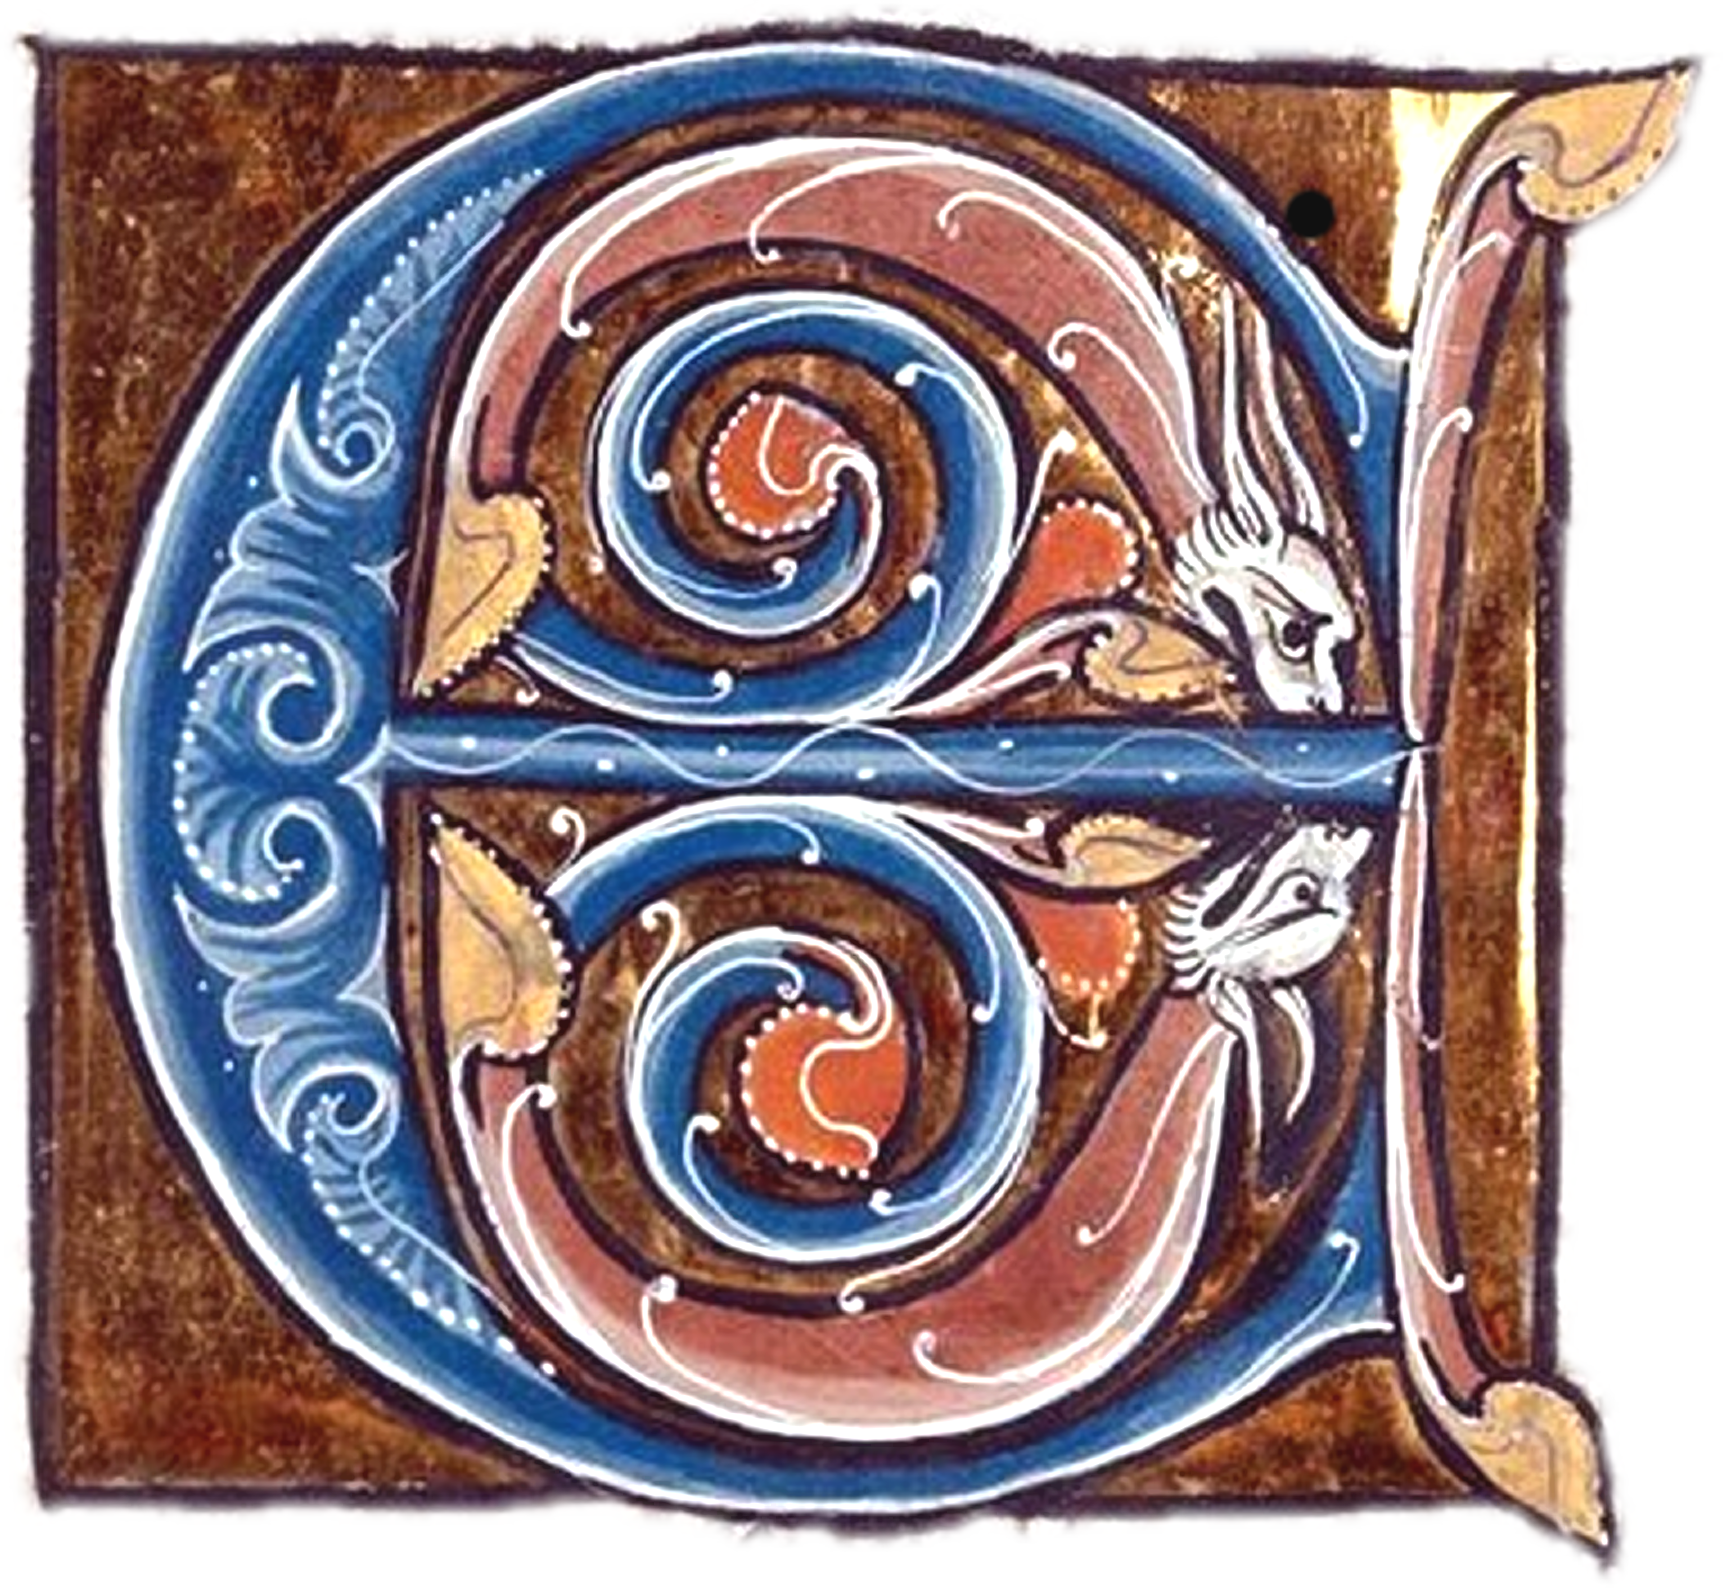
\includegraphics[height=12ex]{img/E0001}}}
\cantus{Introit}{EcceAdvenit}{Intr.}{2.}%
}

\cantus{Graduel}{OmnesDeSaba}{Grad.}{5.}

\cantus{Alleluia}{VidimusStellam}{}{2.}

%\pagebreak
\cantus{Offertoire}{RegesTharsis}{Off.}{5.}

\cantus{Communion}{VidimusStellam}{Comm.}{4.}

\textbf{\begin{center}{Vigile pascale}\end{center}}
\cantus{Fleuris}{Ep_Paques_nuit}{Col}{3, 1-4}
%\begin{center}\textsc{Lecture de l'épître de saint Paul aux Colossiens}\end{center}
%\emph{\color{black} Mes Frères, Si vous êtes ressuscités avec le Christ, recherchez les choses d’en haut, là où le Christ est assis à la droite de Dieu ; goûtez les choses d’en haut, et non celles de la terre ; car vous êtes morts, et votre vie est cachée avec le Christ en Dieu. Quand le Christ, votre vie, apparaîtra, alors vous apparaîtrez vous aussi avec lui dans la gloire.}

\newpage
\textbf{\begin{center}{Jour de Pâques}\end{center}}

\cantus{Fleuris}{Ep_Paques_jour}{I Co}{5, 7-8}
%\bigskip
%\begin{center}\textsc{Lecture de l'épître de saint Paul aux Corinthiens}\end{center}
%\smallskip
%\emph{\color{black} Mes frères, purifiez-vous donc du vieux levain, afin que vous soyez une pâte nouvelle, comme vous êtes des azymes. Car notre agneau pascal, le Christ, a été immolé. C’est pourquoi, mangeons la pâque, non avec un vieux levain, ni avec un levain de malice et de perversité, mais avec des azymes de sincérité et de vérité.}
%{\centering \textbf{Commune Confessoris\\non Pontificis. II.}\par}
\chead{\rubrum Comm. Conf. non Pontificis. II.}

\bigskip

\cantus{Introit}{IustusUtPalma}{Intr.}{1.}%

\cantus{Graduel}{OsIusti}{Grad.}{1.}

\needspace{.3\paperheight}
\cantus{Alleluia}{BeatusVirQuiTimet}{}{5.}

\needspace{.3\paperheight}
\cantus{Offertoire}{InVirtuteTua}{Off.}{6.}

\cantus{Communion}{AmenDicoVobisQuodVos}{Comm.}{1.}

\end{document}
